\documentclass[12pt]{article}
\usepackage{amsmath,amssymb,amsthm}
\usepackage{graphicx}
\usepackage{hyperref}
\usepackage{listings}
\usepackage{float}
\usepackage{tabularx}
\usepackage{multirow}
\usepackage{tikz}
\usepackage{algorithm}
\usepackage{algorithmic}

% Custom environments
\newenvironment{hodos}{\begin{quote}\itshape}{\end{quote}}
\newtheorem{principle}{Principle}
\newtheorem{governance}{Governance Rule}

% Listings configuration for RIFT syntax
\lstdefinelanguage{rift}{
  keywords={let, type, align, span, if, else, policy, token},
  keywordstyle=\color{blue}\bfseries,
  commentstyle=\color{green},
  stringstyle=\color{red},
  morecomment=[l]{//},
  morecomment=[s]{/*}{*/}
}

\title{The RIFT Architecture: A Flexible Translator for Quantum-Deterministic Computation}
\author{OBINexus Project\\
Nnamdi Michael Okpala}
\date{\today}

\begin{document}
\maketitle

\begin{abstract}
RIFT (RIFT is a Flexible Translator) is a revolutionary compiler toolchain designed to bridge classical and quantum computation through deterministic entropy distribution and policy-governed memory management. Born from the necessity of safety-critical system transparency—specifically a failed sleep apnea device—RIFT enforces governance over chaos through a stage-bound execution pipeline, token triplet architecture, and quantum byte standardization. This document formalizes the complete RIFT ecosystem, from its core philosophy to its integration with BEC vacuum isolators for the OBINexus warp drive framework.
\end{abstract}

\section{Introduction: From Failure to Philosophy}

\subsection{The RIFTer's Way}
\begin{hodos}
\textbf{Governance over Chaos}: Every system must be governed, not guessed. Policies must be explicit.\\[0.5em]
\textbf{Intention Embedded}: Code reflects purpose. Bytecode should express the same truth as the source.\\[0.5em]
\textbf{Safety as First-Class Citizen}: Thread safety, memory safety, and user safety are not afterthoughts.\\[0.5em]
\textbf{Careful Binding}: Bindings are acts of care, not control. Drivers must be explicit and traceable.
\end{hodos}

\subsection{What is RIFT?}
RIFT is a flexible translator—a compiler toolchain that transforms the landscape of programming language development. Unlike traditional compiler-compilers like YACC that require months of learning and development, RIFT provides:
\begin{itemize}
\item Configuration-based language development via \texttt{.rift} files
\item Stage-bound execution pipeline with deterministic outcomes
\item Compile-time safety through token triplet architecture
\item Seamless classical-quantum mode transitions
\end{itemize}

\section{System Architecture}

\subsection{Core Components}
\begin{table}[H]
\centering
\caption{RIFT Ecosystem Components}
\begin{tabular}{|l|p{8cm}|}
\hline
\textbf{Component} & \textbf{Specification} \\
\hline
LibRIFT & Pattern-matching engine with regex and isomorphic transforms \\
\hline
RiftLang & Policy-enforced DSL generator with AST management \\
\hline
GossiLang & Polyglot driver system for thread-safe cross-language communication \\
\hline
NLINK & Intelligent linker using automaton state minimization \\
\hline
rift.exe/lrift.so & Compiler/runtime enforcing \texttt{.rift} policies \\
\hline
\end{tabular}
\end{table}

\subsection{Token Triplet Architecture}
\begin{principle}[Token Triplet]
Every RIFT token consists of three components in strict order:
\[
\text{token} = (\underbrace{\text{token\_memory}}_{\text{fluid}}, \underbrace{\text{token\_type}}_{\text{semantic}}, \underbrace{\text{token\_value}}_{\text{concrete}})
\]
\end{principle}

This separation enables compile-time safety by isolating memory allocation from type declaration and value assignment.

\section{Stage-Bound Execution Pipeline}

\subsection{Pipeline Overview}
The RIFT compilation process follows a strict stage-bound execution model:

\begin{figure}[H]
\centering
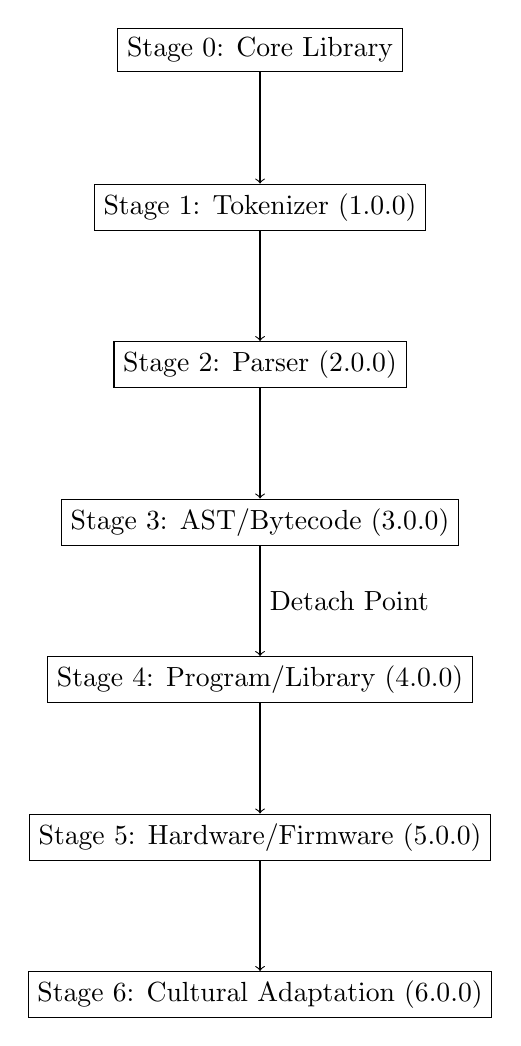
\begin{tikzpicture}[node distance=2cm]
\node[draw,rectangle] (stage0) {Stage 0: Core Library};
\node[draw,rectangle,below of=stage0] (stage1) {Stage 1: Tokenizer (1.0.0)};
\node[draw,rectangle,below of=stage1] (stage2) {Stage 2: Parser (2.0.0)};
\node[draw,rectangle,below of=stage2] (stage3) {Stage 3: AST/Bytecode (3.0.0)};
\node[draw,rectangle,below of=stage3] (stage4) {Stage 4: Program/Library (4.0.0)};
\node[draw,rectangle,below of=stage4] (stage5) {Stage 5: Hardware/Firmware (5.0.0)};
\node[draw,rectangle,below of=stage5] (stage6) {Stage 6: Cultural Adaptation (6.0.0)};

\draw[->] (stage0) -- (stage1);
\draw[->] (stage1) -- (stage2);
\draw[->] (stage2) -- (stage3);
\draw[->] (stage3) -- node[right] {Detach Point} (stage4);
\draw[->] (stage4) -- (stage5);
\draw[->] (stage5) -- (stage6);
\end{tikzpicture}
\caption{RIFT Stage-Bound Execution Pipeline}
\end{figure}

\subsection{Stage Specifications}
\begin{table}[H]
\centering
\caption{RIFT Stage Details}
\begin{tabular}{|c|l|l|l|}
\hline
\textbf{Stage} & \textbf{Name} & \textbf{Version} & \textbf{Output} \\
\hline
1 & Tokenizer & 1.0.0 - 1.1.1 & Token triplets \\
\hline
2 & Parser & 2.0.0 - 2.1.1 & AST nodes \\
\hline
3 & Bytecode & 3.0.0 - 3.1.1 & Opcodes + operands \\
\hline
4 & Program & 4.0.0 & Executable/Library \\
\hline
5 & Hardware & 5.0.0 & Silicon/Firmware \\
\hline
6 & Cultural & 6.0.0 & Localized adaptation \\
\hline
\end{tabular}
\end{table}

\section{Policy System and Error Governance}

\subsection{2×2 Policy Matrix}
\begin{table}[H]
\centering
\caption{RIFT Policy Enforcement Matrix}
\begin{tabular}{|l|l|l|}
\hline
& \textbf{Positive} & \textbf{Negative} \\
\hline
\textbf{True} & True Positive & True Negative (Type II Error) \\
\hline
\textbf{False} & False Positive (Type I Error) & False Negative \\
\hline
\end{tabular}
\end{table}

\subsection{Error Zone Management}
\begin{equation}
\text{Error Zones} = \begin{cases}
0-3 & \text{OK Zone (Detach allowed)} \\
3-6 & \text{Warning Zone (Danger imminent)} \\
6-9 & \text{Critical Zone (Many errors)} \\
9-12 & \text{Panic Zone (System quit)} \\
>12 & \text{Extended trace (no-panic flag)}
\end{cases}
\end{equation}

\section{R Syntax: RIFT Regular Expressions}

\subsection{Expression Format}
RIFT introduces R syntax for pattern matching:
\begin{lstlisting}[language=rift]
r"[^a-z][^0-9]\b"gmit
\end{lstlisting}

Components:
\begin{itemize}
\item \texttt{r""}: RIFT regex declaration
\item \texttt{[\^{}a-z]}: Match anything not a-z
\item \texttt{[\^{}0-9]}: Match anything not 0-9
\item \texttt{\textbackslash b}: Boundary marker
\item \texttt{g}: Global matching
\item \texttt{m}: Multi-line
\item \texttt{i}: Case insensitive
\item \texttt{t}: Top-down parser
\item \texttt{b}: Bottom-up parser
\end{itemize}

\section{Quantum Mode Integration}

\subsection{BEC Vacuum Isolator}
Based on your specifications for absolute zero qubit freezing:

\begin{principle}[BEC Isolation]
The BEC (Bose-Einstein Condensate) creates a super-condensed vacuum chamber where:
\begin{itemize}
\item Temperature: $T < 50$ pK (absolute zero approach)
\item State: Frozen superposition with no interaction capability
\item Purpose: Void engine for deterministic quantum computation
\end{itemize}
\end{principle}

\begin{equation}
\boxed{
\text{BEC State} = \lim_{T \to 0} \langle \hat{H}_{\text{kin}} \rangle = 0
}
\end{equation}

\subsection{Quantum Byte Standard}
Each quantum byte consists of 8 qubits with structured entropy distribution:

\begin{lstlisting}[language=Python, caption=Quantum Byte Allocator]
class QuantumByteAllocator:
    def __init__(self):
        self.qubit_count = 8
        self.entropy_threshold = 0.25
        
    def allocate(self, quantum_state):
        """Allocate 8-qubit quantum byte with entropy balancing"""
        qubits = [self.create_qubit() for _ in range(8)]
        
        # Balance entropy across all qubits
        for i, qubit in enumerate(qubits):
            entropy_weight = exp(-beta * E_i / (k_B * T))
            qubit.apply_entropy_weight(entropy_weight)
            
        return QuantumByte(qubits)
\end{lstlisting}

\section{Implementation Roadmap}

\subsection{Development Stages}
\begin{hodos}
\textbf{Stage 1: Core Governance}: Implement preprocessing policy enforcement\\[0.5em]
\textbf{Stage 2: Quantum Byte Standard}: Develop 8-qubit memory allocator\\[0.5em]
\textbf{Stage 3: Syntax Translation}: Build BitLexPolicy for mode interoperability\\[0.5em]
\textbf{Stage 4: BEC Integration}: Implement vacuum isolator protocol\\[0.5em]
\textbf{Stage 5: Detach Mode}: Enable autonomous language development
\end{hodos}

\subsection{Compilation Example}
\begin{lstlisting}[language=bash]
# Standard RIFT compilation
$ gcc -lriftlang -o threaded_safe_program \
      src/*.c include/*.h policy.rift

# Detach mode configuration
$ ./rift.exe --config go.rift.311.xml --detach
\end{lstlisting}

\section{Conclusion}
RIFT represents a paradigm shift in compiler design, transforming months of language development into configuration-based specification. By enforcing governance through explicit policies and maintaining compile-time safety through token triplets, RIFT enables developers to create domain-specific languages with unprecedented speed and reliability. The integration with quantum computing through BEC vacuum isolation and structured entropy distribution positions RIFT as the foundational technology for the OBINexus warp drive control system.

\appendix
\section{RIFT Command Reference}
\begin{table}[H]
\centering
\begin{tabular}{|l|l|}
\hline
\textbf{Command} & \textbf{Description} \\
\hline
\texttt{rift.exe} & Main compiler executable \\
\hline
\texttt{rift-test.exe} & Testing framework \\
\hline
\texttt{gossi.exe} & GosiLang runtime \\
\hline
\texttt{--detach} & Enable detach mode \\
\hline
\texttt{--no-panic} & Disable panic on critical errors \\
\hline
\end{tabular}
\end{table}

\end{document}